\documentclass{article}

% The following \documentclass options may be useful:

% preprint      Remove this option only once the paper is in final form.
% 10pt          To set in 10-point type instead of 9-point.
% 11pt          To set in 11-point type instead of 9-point.
% authoryear    To obtain author/year citation style instead of numeric.
\usepackage[hmargin=2cm,vmargin=1.5cm]{geometry}
\usepackage{amsmath}
\usepackage{epsfig,times}
%\usepackage{algorithm}
%\usepackage{algorithmicx,algpseudocode}
\usepackage[linesnumbered, ruled]{algorithm2e}
\SetKwRepeat{Do}{do}{while}%
%\usepackage[ruled]{algorithm2e}
%\usepackage{algorithmic,algorithm2e,float}
\usepackage{float}
\usepackage{listings}
\usepackage{color}
\usepackage{graphicx}

\usepackage{listings}
\usepackage{color}

%
% By default LaTeX is quite picky with float placement,
% relax a bit in order to keep this document within 2 pages
%
\renewcommand{\topfraction}{0.95}
\renewcommand{\bottomfraction}{0.95}
\renewcommand{\textfraction}{0.05}
\renewcommand{\floatpagefraction}{0.35}

\lstnewenvironment{code}[1][]%
  {\minipage{\linewidth} 
   \lstset{basicstyle=\ttfamily\footnotesize,frame=single,#1}}
  {\endminipage}

\definecolor{theWhite}{gray}{0.9}
\definecolor{theBlack}{gray}{0.0}
\newcommand{\be}{\begin{equation}}
\newcommand{\ee}{\end{equation}}
\newcommand{\bi}{\begin{itemize}}
\newcommand{\ei}{\end{itemize}}
\newcommand{\eps}{\epsilon}

\begin{document}

\special{papersize=8.5in,11in}
\setlength{\pdfpageheight}{\paperheight}
\setlength{\pdfpagewidth}{\paperwidth}


\title{MLEMV: A R Package for Maximum Likelihood Estimation of Multi-variate Diffusion Models}

\author{Matthew Dixon\\
           Stuart School of Business\\
	   Illinois Institute of Technology\\
           mdixon7@stuart.iit.edu}

\maketitle
\begin{abstract}
Continuous-time Markov
processes are typically defined by stochastic differential equations, describing the evolution of one or more state variables.
Maximum likelihood estimation of the model parameters to historical observations is only possible when at least one of the state variables is observable. In these cases, the form of the transition function corresponding to the stochastic differential equations must be known to assess the efficacy of fitting a continuous model to discrete samples.  This paper describes a R package \verb|MLEVD| for calibrating multi-variate diffusions models.
\end{abstract}


\section{Introduction}
Continuous-time Markov
processes are typically defined by stochastic differential equations, describing the evolution of one or more state variables.
Maximum likelihood estimation of the model parameters to historical observations is only possible when at least one of the state variables is observable. In these cases, the form of the transition function corresponding to the stochastic differential equations must be known to assess the efficacy of fitting a continuous model to discrete samples.  


\cite{Sahalia2002} provide closed form expansions for the likelihood function of a general class of univariate diffusion models. The same author lated extended the approach to multi-variate diffusion models \cite{Sahalia2008} and to, in particular, stochastic volatility models \cite{Sahalia2007}. The later work describes an approach when only of the state variables is observed in financial times series and the other state variable is estimated from both the observed state variable and the corresponding at-the-money constant maturity option prices. The approach is applied to the Heston model \cite{HESTON1993}, a model which has received considerable attention in the context of calibration owing to the many practical challenges and material defects. 

[To do: describe other MLE approaches for Heston, e.g. \cite{Mariani2008}]


\cite{MIKHAILOV2003} address the problem of calibrating Heston's stochastic volatility model by providing guidance on how to calibrate the model to a chain of vanilla call option quotes at one instance of time.

[Tao: can you describe why calibrating to the surface of prices is important?]
The authors draw attention to the fact that the calibration procedure is non-trivial -- it is a non-linear programming problem with a non-linear constraint and non-convex objective function. Since multiple local-minima may exist, \cite{MIKHAILOV2003} propose using a combination of global search and local optimizers.  The authors further note that the use of common stochastic algorithms for global search, such as simulated annealing, generally renders the calibration problem more computationally burdensome. The global optimizers that the authors consider include the differential evolution (DE) algorithm and simulated annealing (SA), both of which have been employed elsewhere in the quantitative finance literature~\cite{ARDIA2011}.


The work of A"{i}t-Sahalia provides a more rigorous alternative to calibrating by least squares, replacing a non-smooth, non-convex of non-concave objective function with a smooth convex or concave function. The calibration of the Heston model to at-the-money option prices is not without its own share of numerical stability challenges, in regions where one or more components of the Jacobian vanish. We provide a R package to compute the log likelihood functions of a general class of multi-variate diffusions and the proceed to perform a numerical study of the estimation of the Heston model parameters first applied to simulated option prices and then applied to high frequency time series data. Finally we comment on the extension of this approach to calibrating to the history of the option chain.

\subsection{Overview of Package}

[To do: Describe the purpose of this package.]

\subsection{Maximum Likelihood Estimation}
The  principle  of
maximum   likelihood   estimation
(MLE), originally developed by R.A. Fisher in the
1920s, states that the desired parametric probability distribution is
the one that renders the observed data most probable.  The maximum likelihood estimator (MLE) is the parameter vector value that maximizes the likelihood function.

Let $i$ denote index observations whose values are $x_i$. Let $\mathbf{\theta}\in\mathbb{R}^p$
be a $p$ parameter vector. Let $y\rightarrow f_i(x|\mathbf{\theta})$ be a smooth positive density. Let $X_i$ be independent with density $f_i(\cdot|\mathbf{\theta})$ which are not independent.  

The data is modeled as observed values of $X_i$ for $i\in1,2,\dots,n$. The likelihood function is
\be
\mathcal{L}(\mathbf{\theta})=\sum_{i=0}^n log f_i(X_i | \mathbf{\theta}).
\ee
The first and second partial derivatives of
$\mathcal{L}$
with respect to $\mathbf{\theta}$ are referred to as the score and the Hessian and
are given by
\be
\mathcal{D}(\mathbf{\theta})=\frac{\partial \mathcal{L}}{\partial \mathbf(\theta)}
\ee
and
\be
\mathcal{H}(\mathbf{\theta})_{ij}=\frac{\partial^2 \mathcal{L}}{\partial\theta_i \partial\theta_j}.
\ee




In the absence of model specification error, we first consider the curvature of the log likelihood function at the stationary point. A large curvature represents more confidence in the MLE and hence a lower standard error.  The curvature is represented by the Information matrix - the negative of the
expected value of the Hessian matrix:

\be
[\mathcal{I}(\mathbf{\theta}))] = - \mathbb{E}[\mathcal{H}(\mathbf{\theta})]
\ee
The variance-covariance matrix of the parameter is
 \be
var(\mathbf{\theta}) =  [\mathcal{I}(\mathbf{\theta})]^{-1}.
\ee
The standard errors of the estimator are just the square roots of the
diagonal terms in the variance-covariance matrix.

By the Cramer-Rao Theorem, under certain regularity conditions on the distribution, the variance of any unbiased estimator of a parameter $\mathbf{\theta}$ must be at least as large as
\be
var(\mathbf{\theta})\geq [-\mathbb{E}[\mathcal{H}(\mathbf{\theta})]^{-1}.
\ee
This theorem implies that the maximum likelihood estimator is efficient but are our assumption is that the data is generated from the model is too strong.


\subsection{Huber Sandwich Estimator}

If the model is not well-specified but the mean function is correctly specified and the variance
function is reasonably specified, then maximum likelihood is asymptotically normal with the
following variance-covariance matrix
\be
var(\mathbf{\hat{\theta}})= [\mathcal{I}(\hat{\mathbf{\theta}})]^{-1}\mathbb{E}[\mathcal{D}(\hat{\mathbf{\theta}})\mathcal{D}(\mathbf{\hat{\theta}})^T][\mathcal{I}(\mathbf{\hat{\theta}}}]^{-1}.
\ee
This is the variance-covariance matrix that provides whose square root of the diagonals provide the robust standard error estimates that are asymptotically correct even when the model is mis-specified. This is the maximum likelihood analogue of White?s consistent standard errors. 

\subsection{Diffusion Models}

Following \cite{Sahalia2002}, consider the multivariate time-homogenous Markovian diffusion of the form
\be
d\mathbf{X}_t=\mathbf{\mu}(\mathbf{X}_t)dt + \Sigma(\mathbf{X}_t)d\mathbf{W}_t
\ee
where $\mathbf{X}_t, \mathbf{\mu} \in \mathbb{R}^m$, $\Sigma(\mathbf{X}_t)\in\mathbb{R}^{m\times m}$ and $\mathbf{W}_t\in \mathbf{R}^m$ are independent Wiener processes.

Prior to the pioneering work of \cite{Sahalia2002}, the log of the transition function $f_X(x|x_0, \Delta)$ was only given in closed form under severe restrictions on the form of $\mathbf{\mu}$ and $\Sigma$. We shall refer the variance-covariance matrix $v(x):=\Sigma\Sigma^T$. \cite{Sahalia2002} constructs closed form expansions for the log-transition function for a large class of multivariate Markovian diffusions. The primary use of such closed form expansions is to permit the computation of the MLE rather than rely on less desirable approaches to inferring the log transition function numerically by solving a partial differential equation, simulating the process to Monte
Carlo integrate the transition density or approximating the process with binomial trees.

We observe $X$ at times $t_0,t_1,\dots,t_n$, where $\Delta$ denotes the difference between observation times and is assumed independent. Under this finite data, the log-likelihood takes the form:
\be
l_n(\mathbf{\theta}, \Delta) :=\sum_{i=1}^n l_X(x_{i+1}|x_i, \Delta),
\ee
where the log of the transition density $l_X:= ln f_X$. Under a Hermite expansion of $l_X$ and application of a number of transformations, \cite{Sahalia2002} eventually arrive at the following compact closed form expression with K terms.
\be
l^(K)_X(x|x_0) = -\frac{m}{2} ln(2\pi\Delta) - D_v(x) + \frac{C_X^{-1}(x|x_0)}{\Delta} + \sum_{k=0}^K C_X^{(k)}(x|x_0)\frac{Delta^k}{k!},
\label{eq:likelihood}
\ee
where
\be
D_v:=-\frac{1}{2}ln(Det[v(x)]).
\ee


%example application to the u3 model

% results - plot, converge, 
% Heston

\subsection{Geometric Brownian motion}

\be
dX_t = \mu X_dt + \sigma X_t dW_t
\ee

\be
f_X(x|x_0,t) = \frac{1}{\sqrt{2\pi}\sigma t}\exp{-\frac{(ln X_t  - ln X_0 - (\mu -\sigma^2/2)t)^2}{2\sigma^2t}}
\ee

\be
l_n(\mathbf{\theta}, \Delta) :=\sum_{i=1}^n l_X(x_{i+1}|x_i, \Delta)=-\frac{1}{2}\sum_{i=1}^{n-1}(ln(2\pi\Delta\sigma^2x_{i+1}^2) + (ln[X_{i+1}/X_{i}] - (\mu-\sigma^2/2)\Delta))^2/(\sigma^2\Delta)
\ee

\subsection{Results}

\begin{figure}
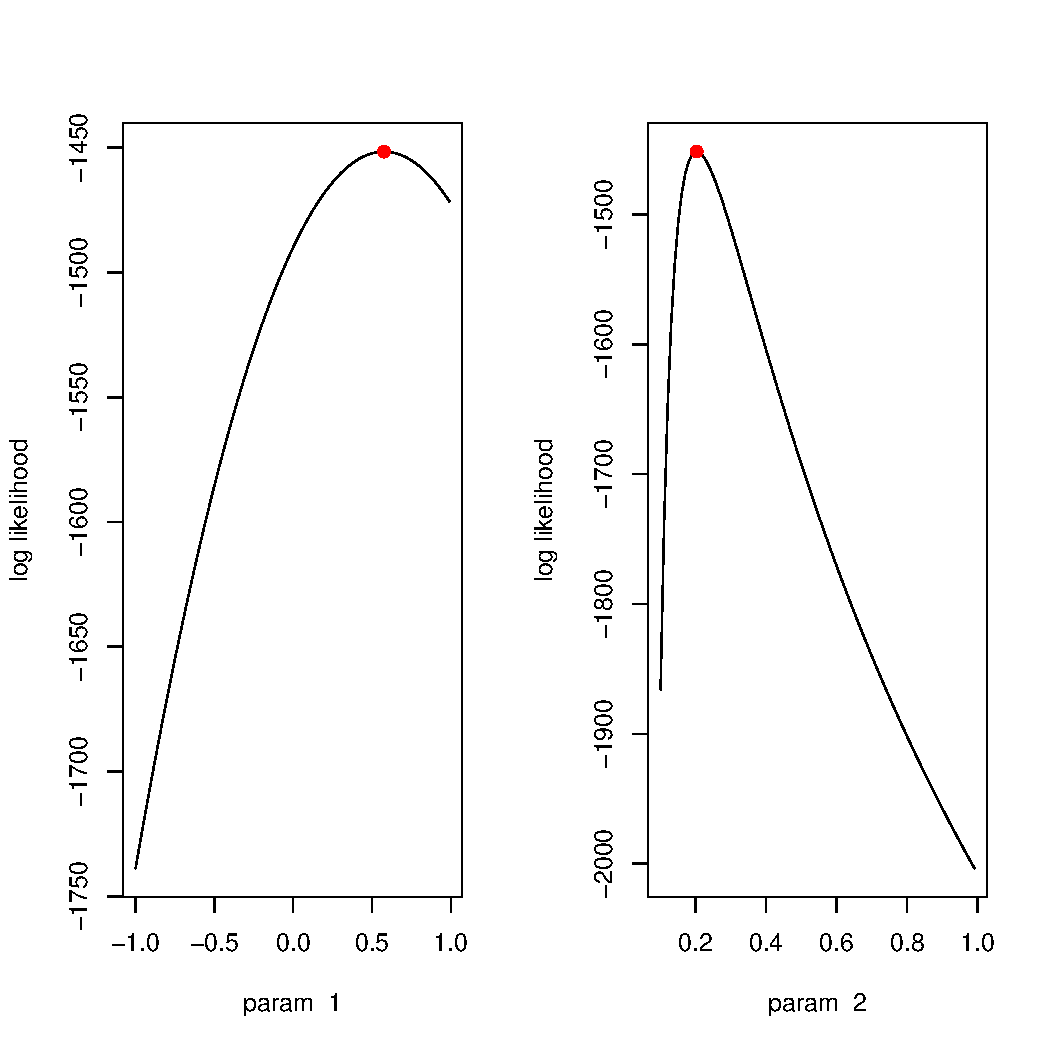
\includegraphics[scale=0.8]{../figures/MLE_GBM.pdf}
\caption{Example plot showing the marginal log likelihood function with respect to each parameter of the geometric brownian diffusion model.}
\end{figure}

\begin{table}[h!]
\begin{tabular}{cc}
Maximum log likelihood & -1309.06362308552\\
Standard Error Estimate &  0.0641498144626433\\
Standard Error Estimate  & 0.00597536567361609\\
Huber Sandwich Error Estimate & 0.064200121510126\\
Huber Sandwich Error Estimate   & 0.00662406799506829\\
Exact Standard Error  & 0.0641498144626433\\
Exact Standard Error  & 0.00597536567361609\\
Exact Huber Sandwich Error &  0.064200121510126\\
Exact Huber Sandwich Error & 0.00662406799506829\\
Error in S.E. Estimate & 5.16892952051595e-13\\
Error in H.S.E. Estimate & 9.33926894153281e-12\\
L2 Norm of Score Error & 1.65901651231863e-07\\
L2 Norm of Hessian Error & 1.44866483253736e-0\\
L2 Norm of Information matrix &  1.96150837439291e-06\\
\end{tabular}
\end{table}

\clearpage

%\subsection{CEV difffusion model}
%
%\be
%dX_t = b(a-x)dt + cx^d dW_t
%\ee


\subsection{Heston Model}\label{sect:heston}

Under the pricing measure $Q$, the Heston model describes the evolution of the log of stock price $s_t =ln~S_t$ whose variance $Y_t$ is given by a mean reverting square root process:
\begin{eqnarray}
ds_t &=& (a + bY_t)dt  + \sqrt{Y_t}dW_1{Q}(t) ,\\
dY_t &=& \kappa'(\theta' - Y_t)dt  + \sigma \sqrt{Y_t}dW_2^{Q}(t),
\end{eqnarray}
where
\be
a=r-d, \qquad b= -\frac{1}{2},
\ee
A key characteristic of the model is that the Wiener processes are correlated $dW^Q_1\cdot dW_2^Q=\rho dt$. This feature enables the model to exhibit the 'leverage effect'. There are five parameters in the model

\begin{itemize}
\item $\kappa$: mean-reversion rate 
\item $\theta$: long-term variance 
\item $\sigma$: volatility of variance 
\item $\rho$: instantaneous correlation between
$dW^Q_1$ and $dW_2^Q$
\item $v_0$: initial variance 
\end{itemize}

%To find the model parameters from option prices first requires adjustment of the model to account for market risk, so that under the objective pricing measure $P$
%\begin{eqnarray}
%ds_t &=& (a + bY_t)dt  + \sqrt{Y_t}dW_1{Q}(t) ,\\
%dY_t &=& \kappa(\theta- Y_t)dt  + \sigma \sqrt{Y_t}dW_2^{Q}(t),
%\end{eqnarray}
%where
%\be
%a=r-d, \qquad b=\lambda_1(1-\rho^2) + \lambda_2\rho -\frac{1}{2}, \qquad \kappa=\kappa'-\lambda_2\sigma, \qquad \theta=\left(\frac{\kappa +\lambda_2\sigma}{\kappa}\right)\theta'.
%a=r-d, \qquad b= -\frac{1}{2}
%\ee

The parameter set $\mathbf{p}:=[\kappa, \theta, \sigma, \rho]$ and the additional non-linear constraint (the Feller condition) $2\kappa\theta - \sigma^2>0$ is imposed during the calibration to ensure that $Y_t$ is positive.

%The parameter set $\mathbf{p}:=[\kappa, \theta, \sigma, \rho, \lambda_1, \lambda_2]$ and the additional non-linear %constraint (the Feller condition) $2\kappa\theta - \sigma^2>0$ is imposed during the calibration to ensure that $Y_t$ is positive.



\subsection{Likelihood function estimation}
Given a set of observed underlying and ATM constant maturity option prices $g_t:=[S_t; C_t]$ sampled at dates $t_0,t_1,\dots, t_n$, the likelihood function takes the form:
\be
l_n(\mathbf{p}):=\frac{1}{n}\sum_{i=1}^nl_G(\Delta t_i,g(t_i)|g(t_{i-1}));\mathbf{p})
\ee
where
\be
l_G(\Delta, g|g_0;\mathbf{p}) := ln f_G(\Delta,g|g_0;\mathbf{p}) = - ln J_t(\Delta, g|g_0;\mathbf{p}) + l_X(\Delta, f^{-1}(g;\mathbf{p})| f^{-1}(g_0;\mathbf{p});\mathbf{p})
\label{eq:likelihood}
\ee
and $l_X$ denotes the likelihood function of the partially observed state vector $x_t:=[ln~S_t, Y_t]$ evaluated at each date $t_0,t_1,\dots, t_n$. Here $\Delta t_i:=t_i-t_{i-1}$ denotes the time step between observations. $J_t$ denotes the Jacobian of the option price with respect to $Y_t$, which is equivalently to vega.


\subsection{Pricing}
With marginal loss of generality, we will restrict the scope of this section to European equity options. The Heston stochastic volatility model permits closed-form solutions for computing risk neutral European option prices. The price can be represented as a weighted sum of the delta of the European call option $P_1$ and $P_2$ - the probability that the asset price will
exceed the strike price at maturity. Adopting standard option pricing notation, the call price of a vanilla European option is
\be
 C(S_0, K,\tau; \mathbf{z}_0) = S_0P_1 - Ke^{-(r-q )\tau}P_2,
\ee
$P_1$ and $P_2$ can be expressed as:
\be \label{eq:p_j}
P_j =\frac{1}{2} + \frac{1}{\pi} \int_{o}^{\infty} \Re\left[\frac{\phi_j (S_0,\tau,u; \mathbf{z}_0)e^{-iu \ln K}}{iu}\right]du, j=1,2.
\ee
where $\phi_j$ are Heston analytic characteristic functions and are given in a convenient form in~\cite{KIENITZ2012}, and $\mathbf{z}_0$ is the vector of Heston model parameters.  Following Fang and Oosterlee~\cite{FANG2008}, the entire inverse Fourier integral in Equation~\eqref{eq:p_j} is reconstructed from Fourier-cosine series expansion of the integrand to give the following approximation of the call price
\be
C(S_0, K, \tau; \mathbf{z}_0) \approx Ke^{-r\tau} \Re\left[\sum_{k=0}^{N-1}\phi\left(\frac{k\pi}{b-a};\mathbf{z}_0\right)e^{ik\pi\frac{x - a}{b-a}}U_k\right],
\ee
where $x:= \ln(S_0/K)$ and $\phi(w;\mathbf{z}_0)$ denotes the Heston characteristic function of the log-asset price, $U_k$ the payoff series coefficients and $N$ denotes the number of terms in the cosine series expansion (typically 128 will suffice).

\subsection{Calibration}

Given a sequence of observed underlying and corresponding near expiry, constant maturity, ATM options, we follow the these steps

\begin{itemize}
\item Initialize the unknown parameter vector to the model
\item For each new parameter set $\mathbf{p}$ generated by the numerical optimization routine, compute the value of $Y_t$ which satisfies the option price. Note this requires solving a nested one dimensional convex optimization, with linear bound constraints, so that $C_t \rightarrow \hat{Y}_t$.
\item With $\hat{Y}_t$ and $\mathbf{p}$ compute $\nu$ of the option and thus the Jacobian term in Equation \ref{eq:likelihood}.
\item Using $\hat{x}_t=[ln~S_t, \hat{Y}_t]$ and $\mathbf{p}$ compute $l_X(\Delta, f^{-1}(g;\mathbf{p})| f^{-1}(g_0;\mathbf{p});\mathbf{p})$
\item Minimize the log likelihood $l_G$ over the parameters subject to the Feller condition. 
\end{itemize}

We implemented the above Algorithm together with the Fourier-Cosine method in R and C++. The Heston price and vega are called by non-linear optimization R packages \verb|NLoptr| and \verb|DEOptim|\cite{Price2006,Ardia2011b}.  More specifically, we combine the \verb|DEOptim| global optimizer with  
one of three constrained local optimization solvers provided in the \verb|NLopt| package. These optimizers are (i) the Sequential Least SQuares Programming (SLSQP) method; (ii) the L-BFGS-B algorithm; and (iii) the Truncated Newton (TNC) method.  Each method exploits the smoothness of the error function over the feasible region by approximating the Jacobian with first order forward differences under perturbations of each parameter.  A small number of Hessian vectors are also computed at each main iteration in the L-BGFS-B algorithm.  The  NLoptr methods described above incorporate the non-linear inequality constraint to enforce the Feller condition.

The number of function evaluations per iteration is thus dependent on the number of model parameters. The global optimizer is terminated if either the objective function is below a threshold or the number of iterations exceeds a limit. The specifiable stopping criterion varies for each of the local optimizers. However, for ease of comparison of convergence properties between each,  it is possible to terminate if either the absolute difference in function values  between successive iterations is within a tolerance or the number of function evaluations exceeds a limit.  In practice, a tolerance on the absolute difference of the function value is neither intuitive or ideally suited to calibration.  In further experiments, not reported here, we find that specifying the tolerance on the norm of the difference in solution iterates leads to more stable parameters over successive calibrations. Of the three aforementioned local solvers, only the TNC method permits a tolerance of this form. 
  
\subsection{Results}

\begin{figure}
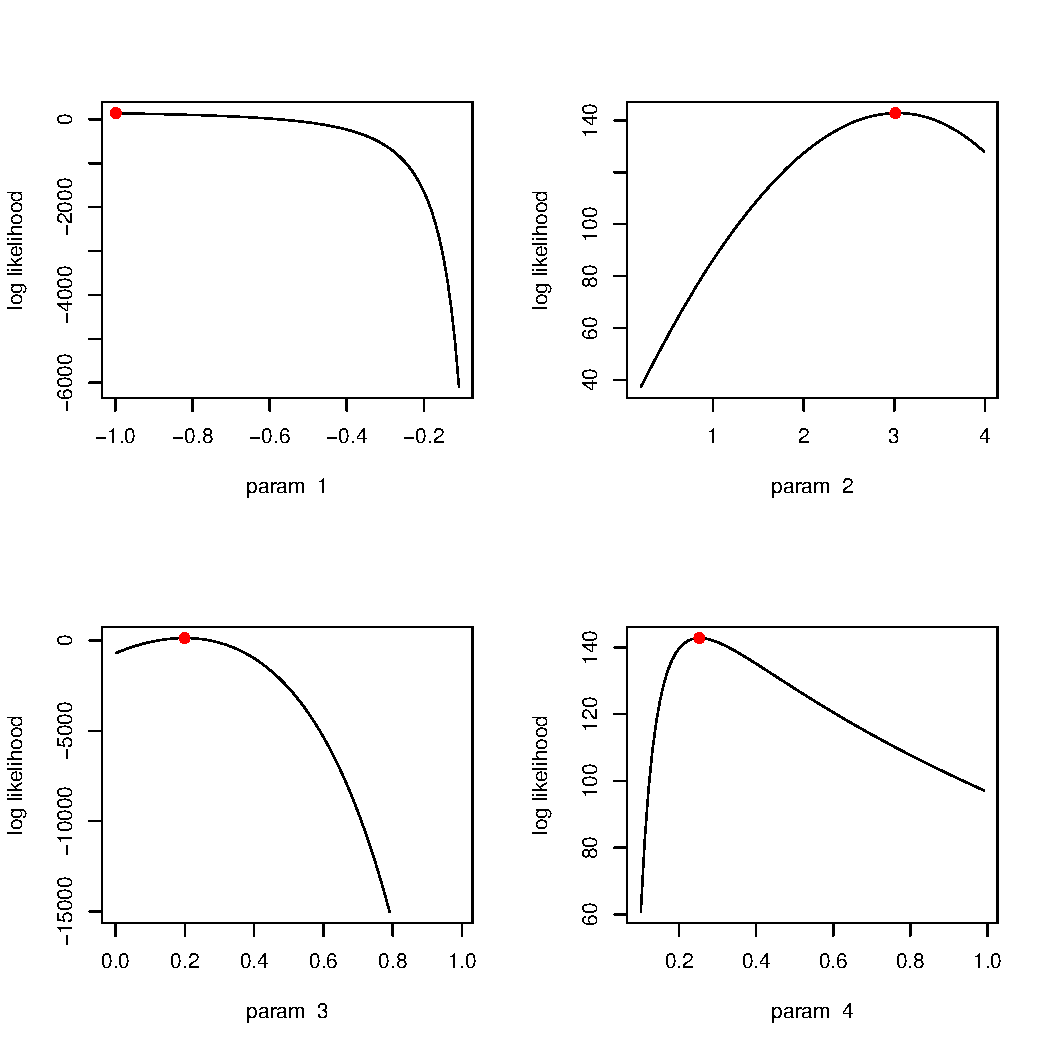
\includegraphics[scale=0.8]{../figures/MLE_Heston.pdf}
\caption{Example plot showing the marginal log likelihood function with respect to each parameter of the Heston model applied to the simulated underlying and prices.}
\end{figure}


[To do: add results calibrating to intra-day atm historical prices]

\clearpage

\appendix
\section{Model Reference}
\begin{table}[h!]
\begin{tabular}{|c|c|c|c|}
\hline
Model & $\mu$ & $\sigma$ & constraints\\
\hline
U1 & $x(a+bx)$ & $\sigma x^{3/2}$ & \\
\hline
U2 & $a+bx$ &$dx$& \\
\hline
U3 & $b(a-x)$ & $cx^d$& \\
\hline
U4 & $\kappa(\alpha-x)$ & $\sigma x^{1/2}& \\
\hline
U5 & $\sum_{i=0}^3 \theta_ix^0$ & \gamma x^\rho$& $\rho\geq 1$\\
\hline
U6 & $a+bx+cx^2+dx^3$ & $f$ & \\
\hlne
U7 & $\kappa(\alpha-x)$ & $\sigma$ & \\
\hline
U8 & $\frac{a_{-1}}{x} + a_0 + a_1x+ a_2x^2$ & $\sigma x^p$ & $\rho\geq 1$\\
\hline
U9 & $\frac{a_{-1}}{x} + a_0 + a_1x+ a_2x^2$ & $(b_0 +b_1x+b_2x^{b_3})^{1/2}$ & \\
\hline
U10 & $\frac{a_{-1}}{x} + a_0 + a_1x+ a_2x^2$ & $b_0 +b_1x+b_2x^{b_3}$ & $\rho\geq 1$\\
\hline
U11 & $a+bx$ & $f+dx$ &\\
\hline
U12 & $\frac{\beta}{x}-\alpha x^3$ & $\gamma x^{1/2}$ & \\
\hline
U13 & $\frac{a_{-1}}{x} + a_0 + a_1x+ a_2x^2 +a_3x^3$ & $\sigma x^{\rho}$ & $\rho\geq 1$\\
\hline
\end{tabular}
\end{table}


\begin{table}[h!]
\begin{tabular}{|c|c|c|c|}
\hline
Model & $\mu(x_1,x_2)$ & $\Sigma(x_1,x_2)$ & constraints\\
\hline
B1 & $\left( \begin{array}{c} a+bx_2\\ c+dx_2 \end{array} \right)$ & $\left( \begin{array}{cc} \rho\sqrt(x_2) & 0\\ h & \sqrt{(1-\rho^2)x_2} \end{array} \right)$ & \\
\hline
B2 & $\left( \begin{array}{c} a_0+a_1x_1+a_2x_2\\ b_0+b_1x_1+b_2x_2 \end{array} \right) &
$\left( \begin{array}{cc} c_0+c_1x_1+c_2x_2 & 0\\ 0 & d_0+d_1x_1+d_2x_2 \end{array} \right)$ & \\
\hline
B3 & $\left( \begin{array}{c} \mu -x_2/2\\ \alpha + \beta x_2 \end{array} \right) &
$\left( \begin{array}{cc} \sqrt{x_2} & 0\\ \sigma\rho x_2^{\gamma} & \sigma \sqrt{1-\rho^2}x^{\gamma}_2 \end{array} \right)$ & \\
\hline
B4 & $\left( \begin{array}{c} a_0+a_1x_2\\ b(a-x_2) + \lambda g x_2^{\beta}\sqrt{a+f(x_2-a)} \end{array} \right) &
$\left( \begin{array}{cc}\sqrt{1-\rho^2}\sqrt{a+f(x_2-a)} & \rho\sqrt{a+f(x_2-a)}\\ 0 & g x^{\beta}_2 \end{array} \right)$ & \\
\hline
B5 & $\left( \begin{array}{c} bx_1\\ c-dx_2 \end{array} \right) &
$\left( \begin{array}{cc} hx_1\sqrt{x_2} & 0\\ g\rho \sqrt{x_2} & g \sqrt{1-\rho^2}\sqrt{x_2} \end{array} \right)$ & \\
\hline
B6 & $\left( \begin{array}{c} m - x_2/2\\ a-bx_2 \end{array} \right) &
$\left( \begin{array}{cc} \sqrt{x_2} & 0\\ \sigma \sqrt{1-\rho^2}\sqrt{x_2} & \sigma \rho\sqrt{x_2} \end{array} \right)$ & $2a> \sigma^2$ \\
\hline
B7 & $\left( \begin{array}{c} 0\\ a_1-a_2x_2 \end{array} \right) &
$\left( \begin{array}{cc} \frac{2x_1}{\gamma\sqrt{x_2}} & \frac{2\eta x_1}{\gamma}\\ 2\sqrt{x_2} & 0 \end{array} \right)$ &  \\
\hline
B8 & $\left( \begin{array}{c} a+bx_1\\ cx_2 \end{array} \right) &
$\left( \begin{array}{cc} dx_1^{\gamma}e^{x_2} & 0\\ 0 & f \end{array} \right)$ &  \\
B9 & $\left( \begin{array}{c} a+bx_1\\ cx_2 \end{array} \right) &
$\left( \begin{array}{cc} dx_1^{\gamma}e^{x_2} & 0\\ 0 & f \end{array} \right)$ &  \\
\hline
B10 & 
$\left( \begin{array}{c} b_1(a_1-x_1)\\ b_2(a_2-x_2) \end{array} \right)$ & 
$\left( \begin{array}{cc} g_1 & 0\\ 0 & g_2\sqrt{x_2} \end{array} \right)$ & 
\\

\hline
B11 & 
$\left( \begin{array}{c} k_1 + k_2x_2\\ \kappa(\theta-x_2) \end{array} \right)$ & 
$\left( \begin{array}{cc} \sqrt{1-\rho^2}\sqrt{x_2} & \rho\sqrt{x_2}\\ 0 & \sigma x_2 \end{array} \right)$ & 
\\

\hline
B12 & 
$\left( \begin{array}{c} ax_1\\ -bx_2 \end{array} \right)$ & 
$\left( \begin{array}{cc} cx_1e^{x_2} & 0\\ dr & d\sqrt{1-r^2} \end{array} \right)$ & 
\\

\hline
B13 & 
$\left( \begin{array}{c} b_{11}(a_1-x_1) + b_{12}(a_2-x_2)\\ b_{21}(a_1-x_1) + b_{22}(a_2-x_2) \end{array} \right)$ & 
$\left( \begin{array}{cc} \sigma_{11} & \sigma_{12}\\ \sigma_{21} & \sigma_{22} \end{array} \right)$ & 
\\

\hline
B14 & 
$\left( \begin{array}{c} k_1(x_2-x_1)\\ k_2(\theta-x_2) \end{array} \right)$ & 
$\left( \begin{array}{cc} \sigma\sqrt{x_1} & 0\\ 0 & \sigma_2\sqrt{x_2} \end{array} \right)$ & 
\\

\hline
B15 & 
$\left( \begin{array}{c} a+bx_1\\ fx_1 + dx_2 \end{array} \right)$ & 
$\left( \begin{array}{cc} \sqrt{x_1} & 0\\ h & \sqrt{1+gx_1} \end{array} \right)$ & 
\\

\hline
B16 & 
$\left( \begin{array}{c} a+bx_1+gx_2\\ d + \eta x_1 + fx_2 \end{array} \right)$ & 
$\left( \begin{array}{cc} \sqrt{x_1} & 0\\ h & \sqrt{x_2} \end{array} \right)$ & 
\\

\hline
B17 & 
$\left( \begin{array}{c} a_{00}-(a_1+a_2x_2)/2+(n_0\sqrt{1-g_1^2} + nu_1g_1)(\sqrt{a_1 + a_2x_2}^{b+d}\\ a_{01}+a_{11}x_2+(nu_1g_{11})(\sqrt{a_1+a_2x_2}^{b+d} \end{array} \right)$ & 
$\left( \begin{array}{cc} \sqrt{1-g_1^2}\sqrt{a_1+a_2x_2} & g_1\sqrt{a_1+a_2x_2}\\ 0 & g_{11}(\sqrt{a_1+a_2x_2})^b \end{array} \right)$ & 
\\

\hline
B18 & 
$\left( \begin{array}{c} b_1x_1\\ a_2+b_2x_2 \end{array} \right)$ & 
$\left( \begin{array}{cc} g_{11}e^{x_1} & 0\\ g_{22}r & g_{22}\sqrt{1-r^2} \end{array} \right)$ & 
\\

\hline
B19 & 
$\left( \begin{array}{c} b_1x_1\\ a_2+b_2x_2 \end{array} \right)$ & 
$\left( \begin{array}{cc} e^{x_2} & 0\\ g_{22}r & g_{22}\sqrt{1-r^2} \end{array} \right)$ & 
\\

\hline
B20 & 
$\left( \begin{array}{c} a_1+b_1x_1\\ a_2+b_2x_2 \end{array} \right)$ & 
$\left( \begin{array}{cc} \sqrt{x_2} & 0\\ gr\sqrt{x_2} & g\sqrt{1-r^2}\sqrt{x_2} \end{array} \right)$ & 
\\

\hline
B21 & 
$\left( \begin{array}{c} a_1(b_1-x_1)\\ a_{21}(b_1-x_1)+a_2(b_2-x_2) \end{array} \right)$ & 
$\left( \begin{array}{cc} \sqrt{x_1} & 0\\ g_{21}\sqrt{x_1} & g_{22}\sqrt{x_1} \end{array} \right)$ & 
\\

\hline
B22 & 
$\left( \begin{array}{c} k_1+k_2x_2\\ k(a-x_2) \end{array} \right)$ & 
$\left( \begin{array}{cc} \sqrt{1-r^2}\sqrt{x_2} & r\sqrt{x_2}\\ 0 & sx_2^b \end{array} \right)$ & 
\\
\hline

\end{tabular}
\end{table}
\clearpage

\bibliographystyle{abbrv}
\bibliography{PackageDescription} 

\end{document}



